\normaltrue \difficilefalse \tdifficilefalse
\correctiontrue
%\UPSTIidClasse{11} % 11 sup, 12 spé
%\newcommand{\UPSTIidClasse}{12}

\exer{Pompe à palettes  $\star$ \label{CIN:02:B2:13:10}}
\setcounter{question}{0}\marginnote{\xpComp{CIN}{02}}%\UPSTIcompetence[2]{B2-13}
\index{Compétence B2-13}\index{Compétence CIN-02}
\index{Pompe à palettes}
\ifcorrection
\else
\marginnote{\textbf{Pas de corrigé pour cet exercice.}}
\fi

\ifprof
\else
Soit le mécanisme suivant. On a $\vect{AO}=e\vect{i_0}$ et $\vect{AB}=\lambda(t)\vect{i_1}$. De plus $e=\SI{10}{mm}$ et $R=\SI{20}{mm}$. Le contact entre \textbf{0} et \textbf{2} en $B$ est maintenu en permanence (notamment par effet centrifuge lors de la rotation de la pompe).
\begin{marginfigure}
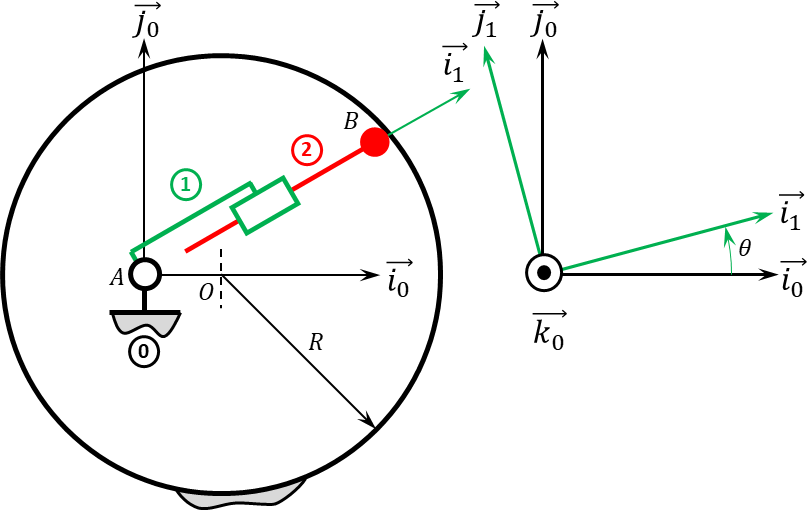
\includegraphics[width=\linewidth]{10_01}
\end{marginfigure}

Il est possible de mettre la loi entrée-sortie sous la forme 
$ \dot{\lambda}_{+}(t)= -e\dot{\theta}(t)\sin\theta(t)-  \dfrac{ e^2\dot{\theta}(t)\cos\theta(t)\sin\theta(t)}{ \sqrt{e^2\cos^2\theta(t)-e^2+R^2}}$
(voir exercice \ref{C2:06:10} -- à vérifier).

\fi


\question{Donner le torseur cinématique $\torseurcin{V}{2}{0}$ au point $B$.}

\ifprof

En utilisant la décomposition du vecteur cinématique, on a :
$\vectv{B}{2}{0} = \vectv{B}{2}{1}+\vectv{B}{1}{0}$.

\begin{itemize}
\item $\vectv{B}{2}{1} = \lambdap(t) \vi{1}$.
\item $\babarv{B}{A}{1}{0}$ $=-\lambda(t)\vi{1}\wedge\thetap(t)\vk{0}$ $=\lambda(t)\thetap(t)\vj{1}$.
\end{itemize}

$\torseurcin{V}{2}{0} = \torseurl{\thetap(t)\vk{0}}{\lambdap(t) \vi{1}+\lambda(t)\thetap(t)\vj{1}}{B}$.

\else
\fi

\question{Déterminer $\vectg{B}{2}{0}$.}

\ifprof

$\vectg{B}{2}{0} = \deriv{\vectv{B}{2}{0}}{\rep{0}}$
$= \lambdapp(t) \vi{1}+\lambdap(t) \thetap(t) \vj{1}+\lambdap(t)\thetap(t)\vj{1}+\lambda(t)\thetapp(t)\vj{1}-\lambda(t)\thetap^2(t)\vi{1} $.


\else
\fi


\ifprof
\else
\footnotesize
\ifcolle
\else
\begin{marginfigure}
\begin{tabular}{|p{.9\linewidth}|}
\hline
Indications :
\begin{enumerate}
\item $\torseurcin{V}{2}{0} = \torseurl{\thetap(t)\vk{0}}{\lambdap(t) \vi{1}+\lambda(t)\thetap(t)\vj{1}}{B}$.
\item $\vectg{B}{2}{0} = \lambdapp(t) \vi{1}+2 \lambdap(t) \thetap(t) \vj{1}+\lambda(t)\thetapp(t)\vj{1}-\lambda(t)\thetap^2(t)\vi{1} $.
\end{enumerate} \\ \hline
\end{tabular}
\end{marginfigure}
\fi

\normalsize
\begin{flushright}
\footnotesize{Corrigé  voir \ref{CIN:02:B2:13:10}.}
\end{flushright}%
\fi